\documentclass{article} % For LaTeX2e
\usepackage{nips12submit_e,times}
%\documentstyle[nips12submit_09,times,art10]{article} % For LaTeX 2.09
\usepackage{amsmath}
\usepackage{algpseudocode}
\usepackage{graphicx}
\usepackage{caption}
\usepackage{subcaption}
\usepackage{natbib}

\title{Formatting Instructions for NIPS 2012}


\author{
David S.~Hippocampus\thanks{ Use footnote for providing further information
about author (webpage, alternative address)---\emph{not} for acknowledging
funding agencies.} \\
Department of Computer Science\\
Cranberry-Lemon University\\
Pittsburgh, PA 15213 \\
\texttt{hippo@cs.cranberry-lemon.edu} \\
\And
Coauthor \\
Affiliation \\
Address \\
\texttt{email} \\
\AND
Coauthor \\
Affiliation \\
Address \\
\texttt{email} \\
\And
Coauthor \\
Affiliation \\
Address \\
\texttt{email} \\
\And
Coauthor \\
Affiliation \\
Address \\
\texttt{email} \\
(if needed)\\
}

% The \author macro works with any number of authors. There are two commands
% used to separate the names and addresses of multiple authors: \And and \AND.
%
% Using \And between authors leaves it to \LaTeX{} to determine where to break
% the lines. Using \AND forces a linebreak at that point. So, if \LaTeX{}
% puts 3 of 4 authors names on the first line, and the last on the second
% line, try using \AND instead of \And before the third author name.

\newcommand{\fix}{\marginpar{FIX}}
\newcommand{\new}{\marginpar{NEW}}

%\nipsfinalcopy % Uncomment for camera-ready version

\begin{document}


\maketitle

\begin{abstract}

\end{abstract}

\section{Introduction}
\label{approach}
Object detection, one of the hard problems in computer vision, has witnessed rapid advancements in both methodology and performance in the past decade. Conceptually, this problem can be viewed on a granularity scale ranging from {\em object class detection} (e.g., being able to detect all types of chairs from training images of some specific chair instances) down to {\em object instance detection} (being able to detect one specific chair based on training images of that chair), and tasks that lie between these two extremes (e.g., being able to detect all Porsche cars or all Porsche 924 models, or all 1976 Porsche 924 instances). For objects with a high degree of visual texture, there have been significant strides in the object instance detection problem using the SIFT features of \cite{Lowe2004} near regions of interesting texture. These methods have led to practical systems that are able to detect hundreds of objects at interactive speeds using GPU acceleration \cite{moped}. 

For less-textured objects, SIFT and similar features are less effective {\bf reference? What is the state of the art in non-textured object instance recognition?}. State of the art object detectors that do not rely on interest points, e.g., \cite{dalal2005histograms,felzenszwalb2008discriminatively,desai2009discriminative} typically build discriminative parametric models based on feature-vectors such as the  HOG features of \cite{dalal2005histograms}, which are strongly view-dependent. This view-dependence coupled with the fact that day-to-day objects themselves have strongly view-dependent visual appearance, means that to apply state-of-the-art methods for non-textured object recognition is a much more difficult problem. Researchers have attempted to account for this view dependence by building multiple parametric  models for different views of the object of interest. Non-parametric methods, or purely data-driven methods, such as \cite{russell2007object,malisiewicz2008recognition}, have not demonstrated superior performance over parametric discriminative methods. One reason might be that the amount of negative data needed in object detection task is enormous and thus hard to represent in non-parametric manner. 


Malisiewicz, et al., presented a method which they called \emph{Exemplar-SVMs} (ESVMs) which builds a single SVM for each positive data instance \emph{(exemplar)} in the training data together with a large collection of negative data \cite{malisiewicz2011ensemble}. ESVM enjoys both discriminative power brought by parametric learning from a large collection of negative samples and the advantages of non-parametric \emph{meta-data transfer} during testing, e.g. segmentation information transfer, 3D information transfer and related object priming \cite{malisiewicz2011ensemble}. Most importantly, the non-parametric aspect allows multiple views of the object to be captured by the model, allowing the method to account for the strong view dependence of most everyday objects. However, \emph{exemplar-based} discriminative methods have difficulty scaling up: both the accuracy and the testing time increase with the number of exemplars. To achieve human-like performance, millions of ESVMs may be required to capture the view variation for some objects, and applying all of them on the testing image becomes impractical. In this paper, we show that this scaling problem for non-textured object recognition can be solved using model recommendation to estimate which models we should apply on the testing image while only actually running a small subset of the total views. This work thus provides a practical method to scale up the exemplar-based object detection system at run time, removing one of the biggest obstacles for practical object instance recognition for non-textured objects.

We formulate our problem as following: given a test image, with an object under an arbitrary viewpoint, detect and classify the object. Instead of the standard testing process used in ESVM (i.e. run all models on that image in a sliding window fashion, followed by applying non-maxima suppression to the detected bounding boxes), we desire to use a small subset of models, which we term \emph{probes} in this paper, to fire on the testing image. Using the responses of these probes, we then use model recommendation to infer which model(s) (in this paper, we refer to them as a \emph{candidate set}) should then be applied to the testing image to get the final detection results. The testing process will be largely speeded up if we can use a small number of \emph{probes} to infer (given that the inference computation is also cheap) which models we should possibly pick for a testing image. 

The concept of using model recommendation in computer vision is not new. Matikainen, et al., \cite{matikainen2012model}, employ model recommendation to perform action recognition in video. Our method differs from Matikainen, et al., in that it focuses on the hard and important problem of scaling up object detection. In particular, the contributions of this paper are as follows: 
\begin{enumerate}
\item We formulate the model recommendation problem for the task of massive multi-view object detection.
\item We show empirically, on four different data sets, that model recommendation can reduce computation time significantly while achieving the same object recognition accuracy.
\item We discuss strategies for selecting good probe sets, and show that surprisingly, for some methods of selecting probes we can achieve accuracy higher than that of using all exemplars on a test image.
\item {\bf other contributions? extensions?}
\end{enumerate}


%For model recommendation, \cite{matikainen2012model} adopted the factor based \emph{collaborative filtering} technique presented in \cite{koren2010factor}, which exploits the structure of the model performance among large amount of models on a small set of data. Based on the assumption that models having a strong relationship with each other (e.g. exemplars for an object instance under different views) and treat the model performance as a rating on a specific task, the collaborative filtering technique is able to find an underlying structure to represent the rating matrix compactly. Different from the goal of standard factor-based collaborative filtering technique, which is to find the underlying latent factors that can best represent the rating results (i.e. fitting every elements), we are aiming at picking out a candidate set which, with large probability, contains models we want to apply. For that, we propose a new matrix factorization method which considers \emph{latent variables} in \emph{high interest region} and relax the original problem to better fit our goal here.\\\\
%In later contents of this section, we briefly review the methodology of Exemplar SVM and the model recommendation. Then we elaborate the proposed high-interest region latent variable collaborative filtering which gives us better performance in our tasks. Finally, the probe selection method is discussed which selects probes for recommendation in a smarter manner instead of selecting randomly.
\section{Approach}
Here we briefly review the Exemplar SVM method and formulate the model recommendation method we use.

\subsection{Exemplar SVM}
\label{exemplarsvm}
Exemplar SVM is trained using only a single object instance and a large collection of negative samples. Since it only uses a single positive instance, the template size could be defined by the instance itself. As suggested by \cite{felzenszwalb2008discriminatively}, the \emph{hard-negative mining} strategy is employed to find negative samples making models more discriminative. More specifically, every object instance is separated from image patches of natural world by drawing a large-margin hyperplane in feature space:

\begin{equation}
\begin{aligned}
\min_{\mathbf{w},b}\frac{1}{2}||\mathbf{w}||^2+C_1l(\mathbf{w},b,\phi(\mathbf{x}_E))+C_2\sum_{\mathbf{x}{\in}\mathcal{N}_E}l(\mathbf{w},b,-\phi(\mathbf{x}))
\end{aligned}
\label{esvmformulation}
\end{equation}

where $\mathbf{x_E}$ is the exemplar and $\mathcal{N}_E$ is the collection of negative samples. $l(\mathbf{w},b,\phi(\mathbf{x}))$ is the hinge loss function evaluated at data point $\mathbf{x}$ using model parameter $\mathbf{w}$ and $b$. $C_1$ and $C_2$ are the constants controlling the amount of penalty put on the penetration of the margin which can be different due to the unbalance number of positive and negative samples. For feature representation of image patch $\mathbf{\phi(x)}$, the \emph{Histogram of Gradient} feature has been demonstrated to be powerful for object detection tasks \cite{dalal2005histograms,felzenszwalb2008discriminatively,malisiewicz2011ensemble}.\\\\
During testing, the learned Exemplar-SVM model $(\mathbf{w},b)$ is applied to the testing image in a sliding-window fashion at varying scales. Then, image patches with responses above a threshold are selected, and non-maxima suppression is applied to get the final detection results.


\subsection{Model Recommendation}
\label{modelrecommendation}
With a large collection of Exemplar-SVM models $\{\mathbf{w}_i,b_i|i=1,2,...,M\}$, when given a testing image $I_t$, the standard way is to run all models in an ensemble way (using the testing strategy described in section \ref{exemplarsvm}). However, applying thousands of models per instance becomes computationally infeasible. This makes ESVMs impractical for building a real-time object detector. \\\\
\emph{Collaborative filtering} (CF), an algorithm for filtering information from various data sources which can be used as components in recommending system, is demonstrated to work as well in recommending models (SVMs) for action recognition \cite{matikainen2012model}. In this paper, we adopt the collaborative filtering as the building block for our model recommending system. \\\\
In order to employ collaborative filtering, we need to pre-compute and store a \emph{collaborative matrix} (also called \emph{rating store} in \cite{matikainen2012model}) which contains results of different models evaluated on different samples. Let $M$ be the total number of models and $N$ be the total number of samples, we evaluate all $M$ models on $N$ samples and get a collaborative matrix $R$:
$$R_{ij}=\max_{\mathbf{x}{\in}I_j}\mathbf{w}_i^T\mathbf{\phi(x)}$$
where $\mathbf{x}$ is an image patch in image $I_j$. $R_{ij}$ is set to be the maximum response of all patches of $I_j$ evaluated by model $\mathbf{w}_i$, as shown in Figure \ref{illus:cm}. Note that different models have different intrinsic popularities which means that some models tend to have higher responses than others consistently, and this unbalance in popularity also applies to different images. Thus, we need to normalize the raw collaborative matrix $R$ to make values in the matrix comparable. In \cite{koren2010factor}, a simple additive model is proposed to represent each value of matrix $R$ as:
$$R_{ij}=\tilde{R}_{ij}+\mu+\alpha_i+\beta_j$$
where $\mu$ is global mean of the matrix $R$, $\alpha_i$ is the representative response for model $i$, and $\beta_j$ is the representative response for image $j$. $\alpha_i$ and $\beta_j$ can be solved as a least square problem by minimizing the square error $\sum_{ij}||R_{ij}-\mu-\alpha_i-\beta_j||^2$. \\\\
Having normalized collaborative matrix $\tilde{R}$, CF discovers the structure in rating matrix by transforming both models (ESVMs) and tasks (images) into a latent factor space. The latent factors try to explain the ratings by characterizing the tasks and models in a lower dimensional space. For example, there might be a dimension in the latent factor space characterizing the angle of viewpoint while another dimension characterizing the illumination condition. The latent factors can be learned by factorizing the collaborative matrix $\tilde{R}$: $\tilde{R}=\Theta^T\Omega$, where $\Theta{\in}\mathbf{R}^{K{\times}M}$ has each column $\phi_i$ to be the latent feature representation for each model, $K$ is the number of latent factors. Similarly, $\Omega{\in}\mathbf{R}^{K{\times}N}$ has each column $\omega_j$ to be the latent feature representation for each image. To solve the above factorization problem, one way is to use \emph{Singular Value Decomposition} to factorize matrix $\tilde{R}$: $\tilde{R}=UDV^T$. By setting $\Theta^T=U'D'$ and $\Omega=V'^T$ ($U'$ is the first $K$ columns of $U$, $D'$ is the upper-left square matrix with dimension $K$ from $D$ and $V'$ is the first $K$ columns of $V$), we can get the desired factorization. It is possible to discover semantic factors using SVD, as shown in Figure \ref{illus:latent}, the curve is value of the first coordinate of latent factors discovered using SVD, which clearly corresponds to the view angle of exemplars. \\\\
Given a testing image $I$, we select a set of probes $\mathcal{S}_p$ with size $|\mathcal{S}_p|$ (for now, $\mathcal{S}_p$ can be selected randomly, we discuss a more sophisticated probe selection method in \ref{probeselection}) and apply models in $\mathcal{S}_p$ on $I$ to get a probe response vector $\mathbf{p}{\in}\mathbf{R}^{|\mathcal{S}_p|\times1}$. $\mathbf{p}$ is then normalized as $\mathbf{\tilde{p}}=\mathbf{p}-\mu-\mathbf{\alpha}_p-\mathbf{\beta}_p$, where $\mathbf{\alpha}_p=\{\alpha_i|i{\in}\mathcal{S}_p\}$, $\mathbf{\beta}_p=\frac{1}{|\mathcal{S}_p|}\sum_j(p_j-\mu)$.  With $\mathbf{\tilde{p}}$, we can recover the latent feature representation of $I$ by solving the linear system for $\omega_p$:
$$\Theta_p^T\omega_p=\mathbf{p}$$
where $\Theta_p$ contains columns extracted from $\Theta$ corresponding to models in $\mathcal{S}_p$. Multiplying the $\omega_p$ with $\Theta$ we get the normalized estimation $\tilde{r}_p$. Using the following formula could we recover the final estimation:
$$r_p=\tilde{r}_p+\mu+\alpha+\beta_p$$
Given this estimated responses of different models on testing image, ideally we can pick the model that has highest estimated response to run on the testing image and get detection result. However, it turns out that even though the estimation has correct tendency to pick out the desired models, e.g. recommending all frontal view models for a frontal view testing image, it is hard for recommendation system to precisely locate the \emph{best} model. Instead, we choose the top $K$ models to form a candidate set and apply all models in this set on testing image\footnote{In all our experiments, we set $K$ to be 20}.\\\\
As an analogy to the standard collaborative filtering setting, here each row of the collaborative matrix represents the score of each model (user) evaluating on different images (items). The collaborative filtering tries to find the underlying latent factors that can characterize both models and images.
\begin{figure}
    \centering
        \begin{subfigure}[b]{0.3\textwidth}
                \centering
                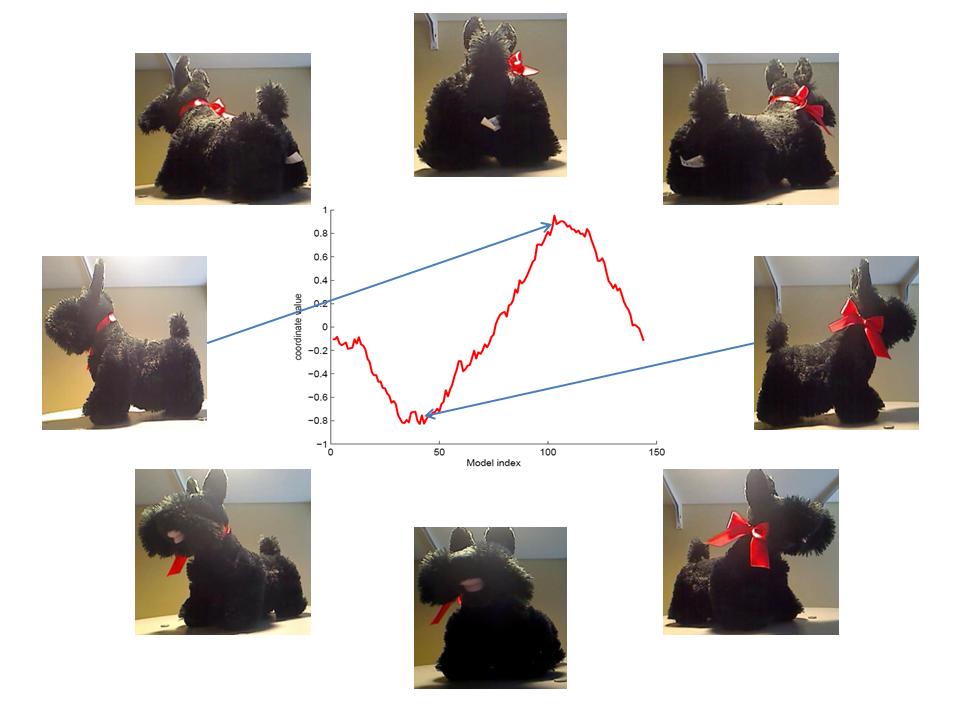
\includegraphics[width=4cm,height=4cm]{fig/latentfactor.png}
                \caption{Illustration of latent factor}
                \label{illus:latent}
        \end{subfigure}
        ~
        \begin{subfigure}[b]{0.3\textwidth}
                \centering
                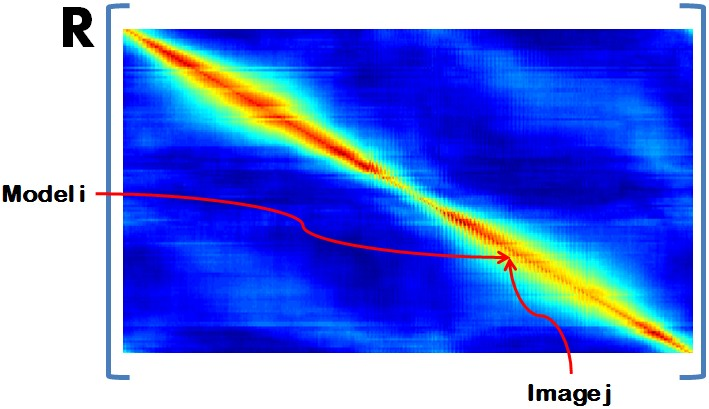
\includegraphics[width=5cm,height=4cm]{fig/matrix.jpg}
                \caption{Collaborative matrix}
                \label{illus:cm}
        \end{subfigure}%
        \caption{\ref{illus:latent} shows the first coordinate of latent factors discovered using SVD. \ref{illus:cm} shows the collaborative matrix}\label{illus}
\end{figure}
\section{Experimental Validation}
\label{evaluation}
To evaluate the effectiveness of model recommendation in object detection task, we conduct experiments on 3 dataset. We have collected a multi-view dataset of a toy dog and recommend models for detecting the target toy in testing sequences which has slight clutter and occlusions. We also apply the proposed method to two public datasets, RGB-D Object Dataset and PASCAL 2007 car dataset \cite{lai2011large,pascal-voc-2007}.
\subsection{Multi-View Toy Dataset}
\begin{figure}
\begin{center}
%\framebox[4.0in]{$\;$}
%\fbox{\rule[-.5cm]{0cm}{4cm} \rule[-.5cm]{4cm}{0cm}}
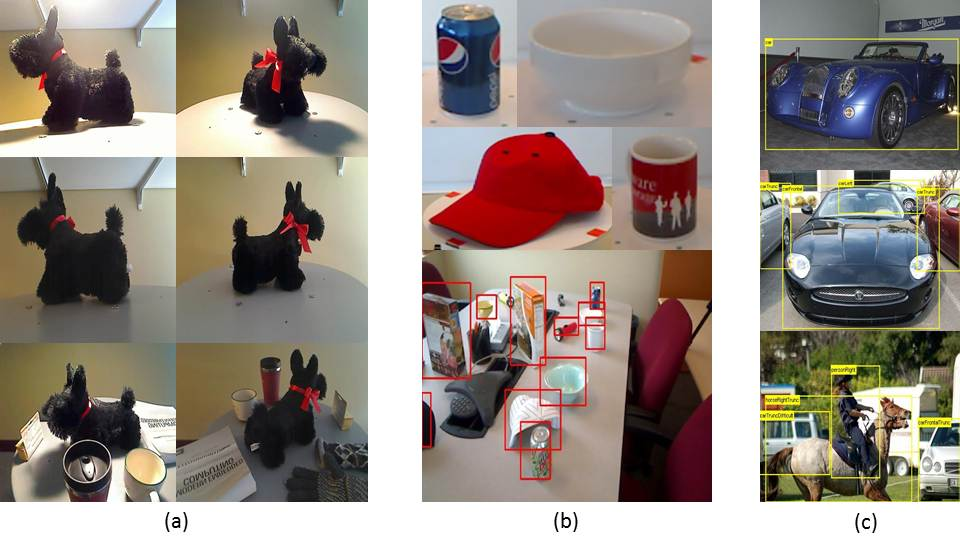
\includegraphics[width=14cm,height=6cm]{fig/figure2total.jpg}
\end{center}
\caption{(a) Examples from Multi-View Toy dataset, the top 2 rows are training images while the last row is from testing sequences. (b) Examples from RGB-D Object Dataset, the top 2 rows are exemplars coming from 4 categories, the bottom row is one frame from testing scene sequence. (c) Sample images from PASCAL car category.}
\label{exampleimages}
\end{figure}

To evaluate the effectiveness of our method, we first focus on the task of detecting a specific instance under arbitrary views with a large collection of models using model recommendation. We collect image sequences by fixing the camera at 5 different arbitrarily chosen height and distance from the toy instance and vary the illumination by turning on/off a lamp above it. The object is set on a turnable table which enables us to collect images for the instance from different views. As a result, we get 10 sequences with frame numbers ranging from 1006 to 1330. For ESVM training, we sample training data from each sequence with rate 2.5 degree/image which leads to 144 exemplars per sequence and consequently 1440 exemplars in total. The collaborative matrix is computed by evaluating all 1440 models on another 4320 images sampled from the training sequences (432 images per sequence) other than images used for training ESVMs. \\\\
For testing, we collect another 2 sequences (with a different height and distance from training samples, one with lamp illumination while another without it) with slight clutters and occlusions. In total there are 1000 images extracted from these two sequences for testing. The typical training and testing data can be seen in Figure \ref{exampleimages}(a). \\\\
To measure the performance of detections, we follow the standard measuring method used in PASCAL object detection challenge \cite{pascal-voc-2007}: all detections are assigned overlapping scores which are intersection areas between estimated bounding boxes and ground truth bounding boxes divided by their union areas. Since this dataset is relatively easy, all detections with overlapping scores higher than 0.7 are considered true positive detection, instead of 0.5 which is used for evaluating performance on PASCAL dataset. We report the average precision (AP), which is an approximation of the area under the precision-recall curve, with regard to the number of models used as probes. For comparison, the baseline is to randomly sample a model subset with the same number of models as probe set and directly apply on testing images. To show how the detection performance approach the standard testing procedure, we also plot out the \emph{best performance} (which we will see not necessarily be the best) which is obtained by applying all models on the testing image. The performance of object detection using recommending system is shown in Figure \ref{curve:multiview}. As shown in the figure, using model recommendation, it is possible to achieve the performance comparable with performance applying all models (the green line) using a very small fraction (5\%) of models due to the correlation among models captured by model recommendation system. The performance curve shown in Figure \ref{curve:multiview} is the average of 100 rounds. The deviations of the average precision at different number of probes are also computed and as we can see from the figure, the deviation for model recommendation is much smaller than our baseline.


\subsection{RGB-D Object Dataset}
The RGB-D Object Dataset is a large data collection consists of 300 daily objects which are categorized into 51 classes. One notable difference between this dataset and classical object dataset like Caltech 101 and ImageNet is that objects in this dataset are separated on two different levels: category level and instance level. For example, for the soda can category, the ground truth labels like \emph{Pepsi Can} and \emph{Mountain Dew Can} are provided in annotation. In our experiment, we focus on instance-level detection task. The cropped object instances for categories \emph{coffee mug}, \emph{soda can}, \emph{cap} and \emph{bowl} are used for this experiment. Note that not all instances are suitable for our model recommendation experiment: some of the objects are quite symmetric and in regular shape which means that the exemplars for this object are highly redundant and the number of models saturate at a small number. The problem of creating a compact model collection is also very interesting though it's beyond the scope of this work. We are interested in objects that have asymmetric appearances and are even deformable to some extent which needs a large collection of models to characterize. Thus, we pick one instance per category\footnote{The index of these four instances are coffee mug \#1, soda can \#1, cap \#4 and bowl \#4} to validate the effectiveness of model recommendation. The instance we choose in each category is shown in top two rows of Figure \ref{exampleimages}b. Since the consecutive frames are very similar, we have sampled images every 5 frames as training data for ESVMs which results in 111, 127, 128 and 118 models of different views for coffee mug, soda can, cap and bowl, respectively. The collaborative filtering matrices for different instances are then computed by evaluating all models belonging to this instance on uncropped images for all these four instances. The precision-recall curves for these four instances are reported in Figure \ref{ap}. Even though our way of measuring performance is different from \cite{lai2011large}, it can still be seen that the exemplar-based method produces quite robust results even using only RGB images without depth information. \\\\
As shown in Figure \ref{curve:RGBDcoffeemug},\ref{curve:RGBDsodacan},\ref{curve:RGBDcap},\ref{curve:RGBDbowl}, for different object instance, model recommendation method requires different amount of probes to achieve a performance comparable with the performance applying all models, this is because that different instances have different variations inspecting from different views and thus make the correlation among models for views vary from instance to instance. However, it is always possible for recommending system to bring us good performance gain over our baseline as shown in the curves. Note that for the bowl instance, model set produced by recommending system actually outperforms the result of applying all models. The reason for this is that model recommendation filters out many false positives when responses among models have strong linear correlation with each other.

\begin{figure}
\begin{center}
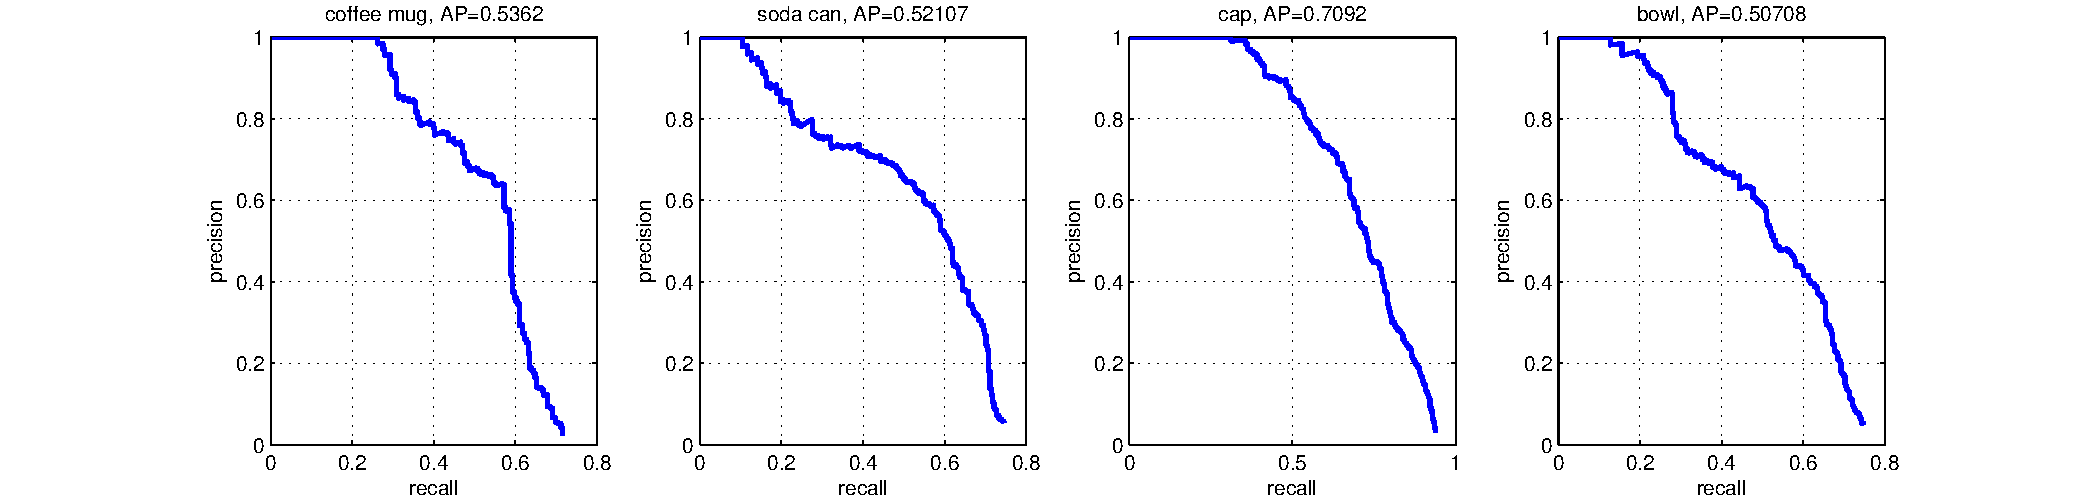
\includegraphics[width=14cm,height=4cm]{fig/apcurve.pdf}
\caption{Precision-recall curve for four selected instances in RGB-D Ojbect Dataset}
\label{ap}
\end{center}
\end{figure}

\begin{figure}
        \centering
        \begin{subfigure}[b]{0.3\textwidth}
                \centering
                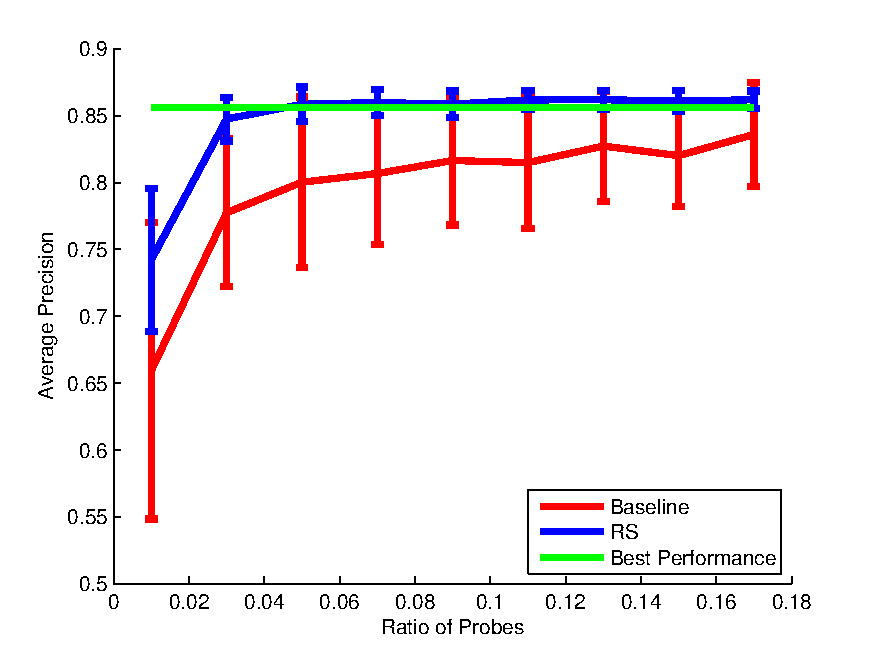
\includegraphics[width=4cm,height=4cm]{fig/multiview.pdf}
                \caption{Multiview Toy}
                \label{curve:multiview}
        \end{subfigure}
        ~
        \begin{subfigure}[b]{0.3\textwidth}
                \centering
                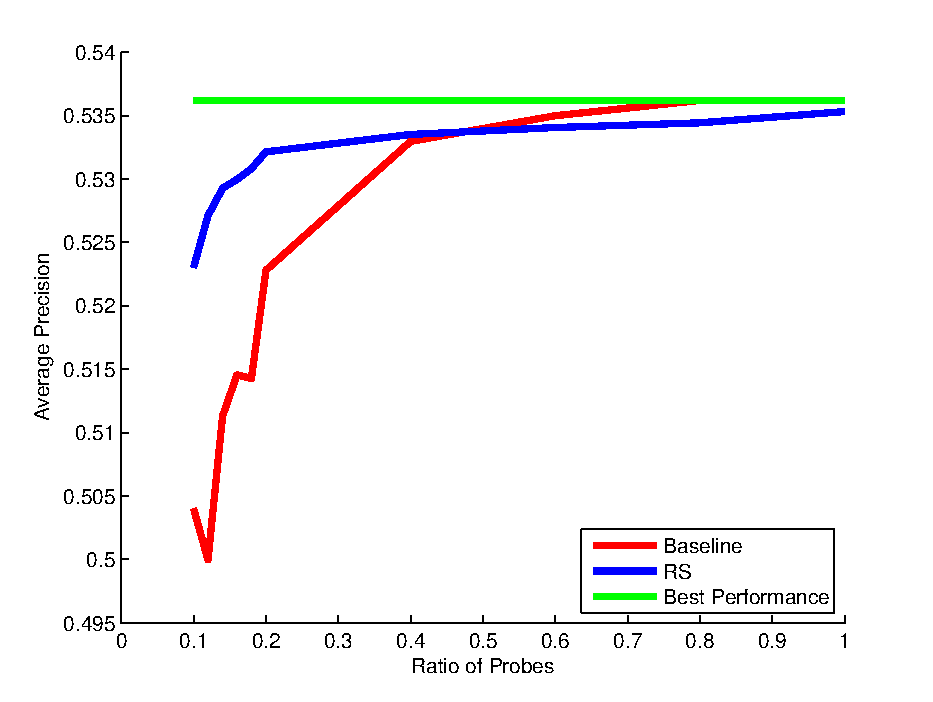
\includegraphics[width=4cm,height=4cm]{fig/coffeemug1pure.pdf}
                \caption{RGBD: coffee mug}
                \label{curve:RGBDcoffeemug}
        \end{subfigure}
        ~
        \begin{subfigure}[b]{0.3\textwidth}
                \centering
                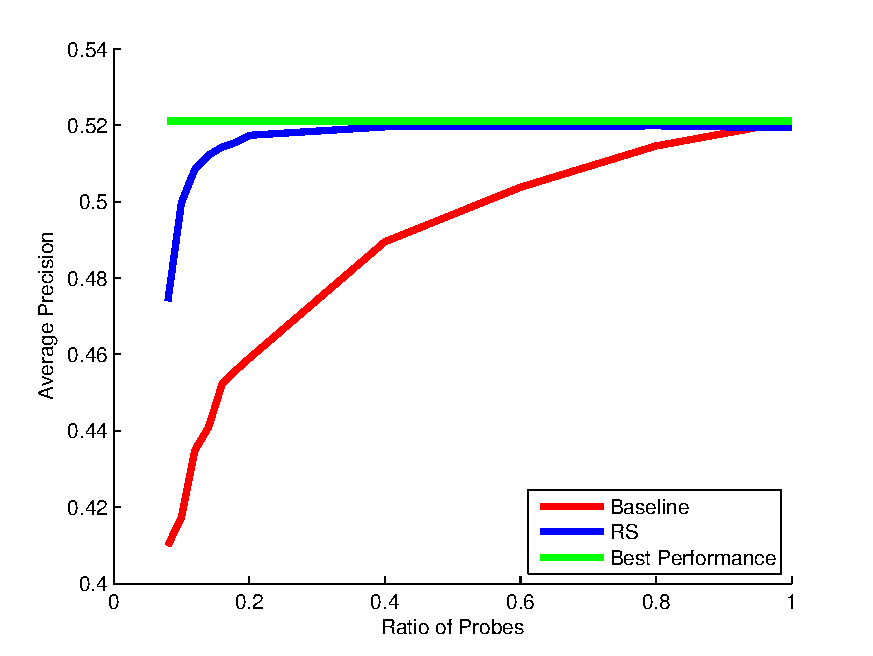
\includegraphics[width=4cm,height=4cm]{fig/sodacan1pure.pdf}
                \caption{RGBD: soda can}
                \label{curve:RGBDsodacan}
        \end{subfigure}

        \begin{subfigure}[b]{0.3\textwidth}
                \centering
                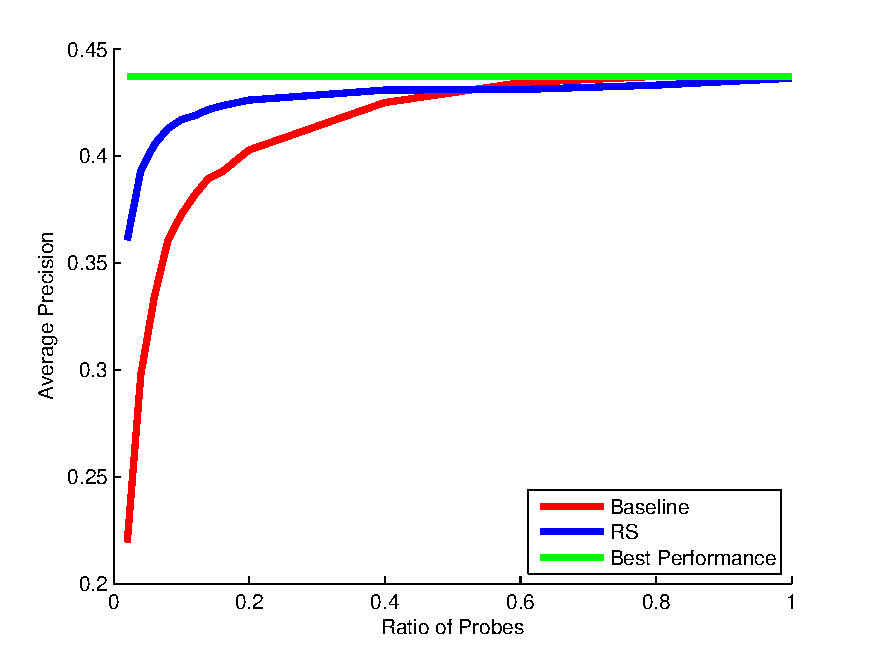
\includegraphics[width=4cm,height=4cm]{fig/pascalcarpure.pdf}
                \caption{PASCAL Car}
                \label{curve:PASCALCAR}
        \end{subfigure}
        ~
        \begin{subfigure}[b]{0.3\textwidth}
                \centering
                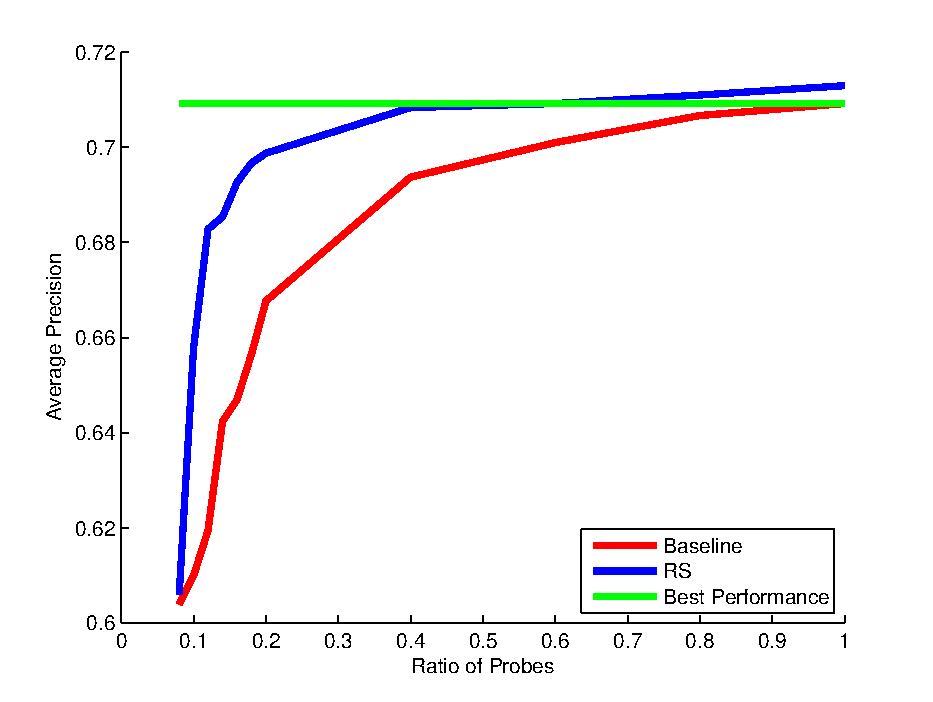
\includegraphics[width=4cm,height=4cm]{fig/cap4pure.pdf}
                \caption{RGBD: cap}
                \label{curve:RGBDcap}
        \end{subfigure}
        ~
        \begin{subfigure}[b]{0.3\textwidth}
                \centering
                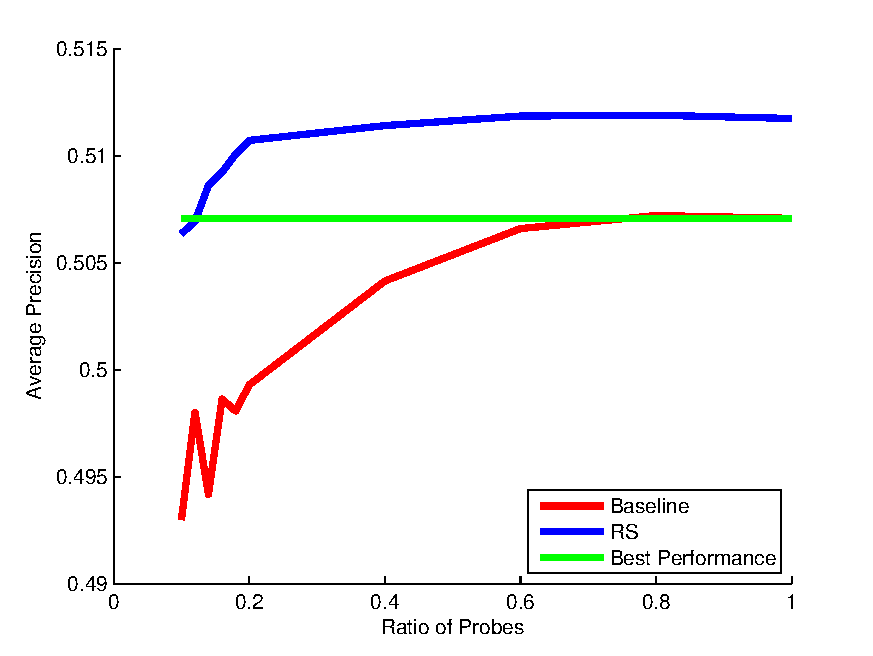
\includegraphics[width=4cm,height=4cm]{fig/bowl4pure.pdf}
                \caption{RGBD: bowl}
                \label{curve:RGBDbowl}
        \end{subfigure}
        \caption{Results for model recommendation, the x-axis is the fraction of models used as probes while the y-axis is the average of average precision over 100 rounds}\label{curve}
\end{figure}



\subsection{PASCAL2007 Car Dataset}
Experiments on Multiview Toy Dataset and RGB-D Object Dataset demonstrate the capability of model recommendation for object instance recognition. We also conduct experiments on PASCAL dataset to see whether the proposed method can generalize to the case of larger variance among models. We use the \emph{car} category in PASCAL 2007 Dataset which includes 1250 instances for different cars from different views with clutters and occlusions. As can be seen from Figure \ref{exampleimages}c, the exemplar models we use in PASCAL Car dataset has much larger variance among models than the models we use in previous experiments. The collaborative matrix is computed by evaluating all models on images from both the \emph{car} and \emph{bus} category in PASCAL dataset. The testing images are taken from PASCAL test set which contain at least one car instance. The result of model recommendation is shown in Figure \ref{curve:PASCALCAR}. We demonstrate that of larger variances among models, the model recommendation is still able to produce comparable detection performance with a relatively small number of probes. \\\\
Experiments on these three datasets consistently demonstrate the capability of model recommendation for object detection. Model recommendation provides a way of reducing the number of models applied to images and thus enables the exemplar set to scale up when detecting objects using exemplars-based method. Under condition where model responses having strong linear correlation, it is even possible for model recommendation to yield better performance than applying all models because it filters out false positive detections.

\section{Extensions (For Now Skip)}
Given the framework of model recommendation, we also explore some possible extensions to further improve the performance from aspects of obtaining latent factors and probe selection.

\subsection{High-Interest Region Latent Variable Matrix Factorization}
In fact, the latent feature representation $\Theta$ and $\Omega$ mentioned in section \ref{modelrecommendation} are obtained by solving the following optimization problem:
\begin{equation}
\begin{aligned}
& \min_{\Theta,\Omega}\frac{1}{2}||\Theta^T\Omega-\tilde{R}||^2_F \\
& \text{subject to    } \Theta,\Omega{\in}\mathcal{O}\\
\end{aligned}
\label{svdformulation}
\end{equation}
$\mathcal{O}$ is the set of orthonormal matrices, $||\cdot||_F$ is the Frobenius norm of a matrix. As we can see from the formulation (\ref{svdformulation}), the objective function aims at minimizing the square error of every elements of the estimated collaborative matrix $\Theta^T\Omega$ from $\tilde{R}$. However, what we are really interested in this scenario is to select a \emph{candidate set} that contains good models (or even the best) for this particular testing image. Also, note that what we are tackling here in the collaborative matrix $R$ are SVM scores, from formulation (\ref{esvmformulation}), we know the absolute value of $R_{ij}$ is the distance between the data point and the hyperplane. We found this quantity to be noisy and sometimes misleading in the sense of measuring how likely the image patch is like the exemplar because of false positive detections. As can be seen in Figure (\ref{HIRLMFprobeselection}a), higher SVM scores do not necessarily imply high overlapping scores. In our formulation, instead of fitting the exact value in $\tilde{R}$ using regression, we relax the problem in high-interest region: values in high-interest region are allowed to vary as long as they are still kept in high-interest region. There are works considering the problem of recommending items to users by paying attentions to item rankings instead of their absolute ``ratings", e.g. \cite{freund2003efficient,cohen1999learning}. Comparing our formulation with ranking-based collaborative filtering technique like \cite{freund2003efficient,cohen1999learning}, note that the key difference between their scenario with ours: in their cases, the ranking output by recommending system will determine the final performance, however in our case, all models in the candidate set will be applied to the testing image and then the \emph{true} SVM score will determine the performance even though it is not consistent with the ranking output by the recommending system (illustrated in Figure (\ref{HIRLMFprobeselection}b)). This property makes our method, which focus on separating ``good" models from ``bad" ones even without considering the ranking within the scope of ``good" models, quite effective in our case. Thus, we define the \emph{high-interest region} $\mathcal{S}_h$ to be the set of elements in matrix $\tilde{R}$ containing top ranking values with set size to be $\rho\cdot|\mathcal{S}_h|$, where $\rho$ is the ratio constant (in our experiments, $\rho$ is empirically set to be 0.01). We denote the threshold (minimum) value in set $\mathcal{S}_h$ to be $V_\rho$. \\\\

\begin{figure}
\begin{center}
%\framebox[4.0in]{$\;$}
%\fbox{\rule[-.5cm]{0cm}{4cm} \rule[-.5cm]{4cm}{0cm}}
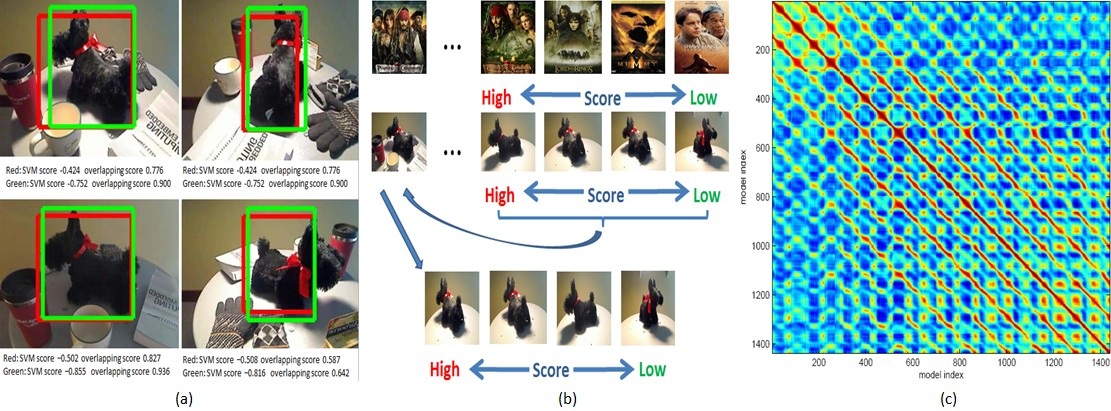
\includegraphics[width=14cm,height=4cm]{fig/figure1total.jpg}
\end{center}
\caption{(a) Illustration for the discrepancy between SVM scores and overlapping scores. (b) Illustration for the difference between our scenario and that of rank-based CF. The top row illustrates scenario of standard collaborative filtering (recommending movies), while the bottom row shows our scenario to recommend model candidate set. (c) Visualization of model correlation.}
\label{HIRLMFprobeselection}
\end{figure}

\textbf{Formulation:} The above motivation can be formulated into the following objective function:

\begin{equation}
\begin{aligned}
& \underset{\Theta,\Omega,\xi}{\text{minimize}}
& & \frac{1}{2}||(\Theta^T\Omega-\tilde{R}){\circ}M_{\mathcal{S}_h}||^2_F+\frac{\gamma_1}{2}||\Theta||_F^2+\frac{\gamma_2}{2}||\Omega||_F^2+C\sum_{(i,j)\in\mathcal{S}_h}\xi_{ij}\\
& \text{subject to}
& & \Theta_i^T\Omega_j{\geq}V_\rho-\xi_{ij}, \forall(i,j){\in}\mathcal{S}_h, \\
\end{aligned}
\label{hirlmf}
\end{equation}
where $\circ$ is the element-wise product, $M_{\mathcal{S}_h}{\in}\mathbf{R}^{M{\times}N}$ is a mask matrix with each element as an indicator showing whether $(i,j)$ pair is in $\mathcal{S}_h$ (i.e. $M_{\mathcal{S}_h}(i,j)=0$, if $(i,j){\in}\mathcal{S}_h$, otherwise $M_{\mathcal{S}_h}(i,j)=1$), $\xi_{ij}$ is the slack variable measuring how much the estimated value penetrate the boundary $V_\rho$. $\gamma_1$, $\gamma_2$ and $C$ are all regularization parameters controlling the complexity of the model. This formulation addresses data in $\tilde{R}$ in two parts. For those elements not in $\mathcal{S}_h$, we fit their values as $\Theta_i^T\Omega_j\rightarrow\tilde{R}_{ij}$. For elements in high-interest region, we assume there to be latent values $\mathcal{L}(i,j)$ that can be better explained by a linear combination of factor elements $\Theta_i$ than the value $\tilde{R}_{ij}$. Actually, the latent variable assumption in high-interest region make the ``collaborative effects" reinforced and we believe the information transfer between different tasks (images) is crucial to prevent from \emph{overfitting} (we will discuss this in detail in section \ref{evaluation}). \\\\
\textbf{Optimization:} The above minimization problem, having an objective function which is in \emph{bi-convex} or more specifically \emph{bi-quadratic} form (being a quadratic form w.r.t one variable when fixing others), can be solved using an \emph{block coordinate descent} algorithm \cite{al1983jointly}. When updating $\Theta_i$, we fix $\Omega$ and all $\{\Theta_k,k{\neq}i\}$. Thus, the objective function reduces as:
\begin{equation}
\begin{aligned}
& \underset{\Theta_i,\xi}{\text{minimize}}
& & \sum_{j,(i,j){\not\in}\mathcal{S}_h}\frac{1}{2}||(\Theta_i^T\Omega_j-\tilde{R}_{ij})||^2+\frac{\gamma_1}{2}||\Theta||_F^2+C\sum_{j,(i,j)\in\mathcal{S}_h}\xi_{ij}\\
& \text{subject to}
& & \Theta_i^T\Omega_j{\geq}V_\rho-\xi_{ij}, {\forall}j,(i,j){\in}\mathcal{S}_h, \\
\end{aligned}
\label{hirlmfsub}
\end{equation}
Using Lagrangian multipliers, we can write down the above optimization problem into its dual form, which is a standard quadratic program with box constraints:
\begin{equation}
\begin{aligned}
& \underset{\alpha}{\text{maximize}}
& & \frac{1}{2}\alpha^TH\alpha+q^T\alpha\\
& \text{subject to}
& & 0\leq\alpha{\leq}C, \\
\end{aligned}
\label{hirlmfdual}
\end{equation}
where $\alpha$ is the dual variable, $H$ and $q$ can be computed using the following equations:
$$q^T=bA^TMA-2bA^TM\Omega_{\mathcal{S}_h}+\lambda_1bA^TM^TM\Omega_{\mathcal{S}_h}+V_\rho\mathbf{1}^T$$
$$H=\Omega_{\mathcal{S}_h}^TM^TAA^TM\Omega_{\mathcal{S}_h}+\lambda_1\Omega_{\mathcal{S}_h}^TM^TM\Omega_{\mathcal{S}_h}-2\Omega_{\mathcal{S}_h}^TM\Omega_{\mathcal{S}_h}$$
$b$ is the vector of $\{\tilde{R}_{ij}|{\forall}j \text{ such that } (i,j)\not\in\mathcal{S}_h\}$, $A=\{\Omega_j|{\forall}j \text{ such that } (i,j)\not\in\mathcal{S}_h\}$, $\Omega_{\mathcal{S}_h}=\{\Omega_j|{\forall}j \text{ such that } (i,j)\in\mathcal{S}_h\}$, $M=(AA^T+\lambda_1I)^{-1}$. \\\\
The $\lambda_1$ in the expression of $M$ makes $M$ invertible. The dual form could then be solved by any quadratic program code, in this paper we adopt the MOSEK which is efficient for large-scale quadratic program with box constraints \cite{mosek}. Note that because of the symmetry of $\Theta$ and $\Omega$, the optimization for $\Omega$ is in the same dual form and we alternate between $\Theta$ and $\Omega$ until convergence. For initialization, we use the same procedure described in section \ref{modelrecommendation} to get initial $\Theta_0$ and $\Omega_0$.


%Applying HIRL matrix factorization yields even better performance than SVD based factorization. The reason for the performance gain becomes obvious if we look at Figure \ref{curve}(b): the horizontal axis is the number of models in probe set while the vertical axis is the proportion of testing images which include the ``best" model (the model yielding the highest response) in the recommended candidate set. HIRL-MF is more powerful in including the best model in its candidate set against SVD-based factorization even though the order of the candidate set is not consistent with the real one. Since in object detection task, the \emph{non-maximum suppression} is applied to reduce the redundant detections, as long as we have the detection from the high-response models in our candidate set, weaker detections will be suppressed and thus not to affect the detection results. The experimental results on this Multi-View Toy dataset validate the effectiveness of model recommendation, OMP probe selection and HIRL-MF.


\subsection{Probe Selection}
\label{probeselection}
It is obvious that different models contain different amount of information for inferring the response estimation. The information one model contains about others could be measured using \emph{sample Pearson correlation coefficient} \cite{lee1988thirteen}. More formally, we treat the response of each model as a random variable $r_i,i=1,2,...,M$ and compute the correlation matrix $\mathcal{C}_{ij}$ as:

\begin{equation}
\begin{aligned}
\mathcal{C}_{ij}=\frac{\sum_{k=1}^N(r_i^{(k)}-\bar{r}_i)(r_j^{(k)}-\bar{r}_j)}{\sqrt{\sum_{k=1}^N(r_i^{(k)}-\bar{r}_i)^2}\sqrt{\sum_{k=1}^N(r_j^{(k)}-\bar{r}_j)^2}}
\end{aligned}
\label{pearson}
\end{equation}

where $\bar{r}_i$ is the empirical mean of $r_i$. If we plot out the matrix $\mathcal{C}$, we can find strong pattern between model outputs (see Figure (\ref{HIRLMFprobeselection}c), which is from the Multi-View Toy dataset we collect for experiment). Dark regions represent strong correlations between models. We don't want to select those models as probes which contain little information (low correlation with other models) about others or those can be estimated quite precisely using models that have already been selected into probe set (redundancies in probe set). To resolve these two problems, we propose to use \emph{orthogonal matching pursuit} to find a sequence which achieves the above two goals \cite{cois1995matching}.\\\\
In initialization step, we normalize the response vector for each model $\tilde{R}_i{\in}\mathbf{R}^{1{\times}N},i=1,2,...,M$ to zero mean and unit length. We initialize two sets $\mathcal{S}_{ps}=\{t\}$ and $\mathcal{S}_r=\{1,2,...,t-1,t+1,...,M\}$, where $t=\arg\max_i\sum_j\mathcal{C}_{ij}$, to be the probe sequence set and the remaining model set, respectively. We denote $\tilde{R}_{ps}$ and $\tilde{R}_r$ the response vectors for the model in $\mathcal{S}_{pr}$ and $\mathcal{S}_r$, respectively. In every iteration, we compute the projections of the remaining model vectors onto the subspace spanned by model vectors in probe set as $p=\text{diag}(\tilde{R}_{r}\tilde{R}_{ps}^T\tilde{R}_{ps}\tilde{R}_r^T)$. $\text{diag}(\cdot)$ is the operator extracting the main diagonal elements as a vector. Then, we add the model index corresponding to the model of the minimum projection length into $\mathcal{S}_{pr}$ and delete it from $\mathcal{S}_r$. The above iterating process terminates until $S_r={\O}$.\\\\
The Pearson correlation coefficient measures the linear correlation between two model responses. The probe sequence generated by OMP aims at spanning the model response space as soon as possible. More specifically, at each step OMP tries to find a probe that is most orthogonal to model response space spanned by current probe set and thus can provide most information. In section \ref{evaluation}, we empirically validate the effectiveness of the OMP probe selection method.


\section{Conclusion}
In this paper, we propose a framework to employ model recommendation for object detection task at run time: a probe set is chosen to be applied on testing image, responses of probes are used to estimate responses of all models on the testing image. A candidate set of models with highest estimated responses are then applied to the testing image to get the final detections. We empirically found that the performance of applying all models can be approached using a small number of probes, which largely speeds up the object detection process. We also show some possible extensions to further improve the performance of model recommendation and show some preliminary results for that.



%\begin{figure}[h]
%\begin{center}
%%\framebox[4.0in]{$\;$}
%\fbox{\rule[-.5cm]{0cm}{4cm} \rule[-.5cm]{4cm}{0cm}}
%\end{center}
%\caption{Sample figure caption.}
%\end{figure}
%
%
%
%\begin{table}[t]
%\caption{Sample table title}
%\label{sample-table}
%\begin{center}
%\begin{tabular}{ll}
%\multicolumn{1}{c}{\bf PART}  &\multicolumn{1}{c}{\bf DESCRIPTION}
%\\ \hline \\
%Dendrite         &Input terminal \\
%Axon             &Output terminal \\
%Soma             &Cell body (contains cell nucleus) \\
%\end{tabular}
%\end{center}
%\end{table}
%
%\section{Preparing PostScript or PDF files}
%
%Please prepare PostScript or PDF files with paper size ``US Letter'', and
%not, for example, ``A4''. The -t
%letter option on dvips will produce US Letter files.
%
%Fonts were the main cause of problems in the past years. Your PDF file must
%only contain Type 1 or Embedded TrueType fonts. Here are a few instructions
%to achieve this.
%
%\begin{itemize}
%
%\item You can check which fonts a PDF files uses.  In Acrobat Reader,
%select the menu Files$>$Document Properties$>$Fonts and select Show All Fonts. You can
%also use the program \verb+pdffonts+ which comes with \verb+xpdf+ and is
%available out-of-the-box on most Linux machines.
%
%\item The IEEE has recommendations for generating PDF files whose fonts
%are also acceptable for NIPS. Please see
%http://www.emfield.org/icuwb2010/downloads/IEEE-PDF-SpecV32.pdf
%
%\item LaTeX users:
%
%\begin{itemize}
%
%\item Consider directly generating PDF files using \verb+pdflatex+
%(especially if you are a MiKTeX user).
%PDF figures must be substituted for EPS figures, however.
%
%\item Otherwise, please generate your PostScript and PDF files with the following commands:
%\begin{verbatim}
%dvips mypaper.dvi -t letter -Ppdf -G0 -o mypaper.ps
%ps2pdf mypaper.ps mypaper.pdf
%\end{verbatim}
%
%Check that the PDF files only contains Type 1 fonts.
%%For the final version, please send us both the Postscript file and
%%the PDF file.
%
%\item xfig "patterned" shapes are implemented with
%bitmap fonts.  Use "solid" shapes instead.
%\item The \verb+\bbold+ package almost always uses bitmap
%fonts.  You can try the equivalent AMS Fonts with command
%\begin{verbatim}
%\usepackage[psamsfonts]{amssymb}
%\end{verbatim}
% or use the following workaround for reals, natural and complex:
%\begin{verbatim}
%\newcommand{\RR}{I\!\!R} %real numbers
%\newcommand{\Nat}{I\!\!N} %natural numbers
%\newcommand{\CC}{I\!\!\!\!C} %complex numbers
%\end{verbatim}
%
%\item Sometimes the problematic fonts are used in figures
%included in LaTeX files. The ghostscript program \verb+eps2eps+ is the simplest
%way to clean such figures. For black and white figures, slightly better
%results can be achieved with program \verb+potrace+.
%\end{itemize}
%\item MSWord and Windows users (via PDF file):
%\begin{itemize}
%\item Install the Microsoft Save as PDF Office 2007 Add-in from
%http://www.microsoft.com/downloads/details.aspx?displaylang=en\&familyid=4d951911-3e7e-4ae6-b059-a2e79ed87041
%\item Select ``Save or Publish to PDF'' from the Office or File menu
%\end{itemize}
%\item MSWord and Mac OS X users (via PDF file):
%\begin{itemize}
%\item From the print menu, click the PDF drop-down box, and select ``Save
%as PDF...''
%\end{itemize}
%\item MSWord and Windows users (via PS file):
%\begin{itemize}
%\item To create a new printer
%on your computer, install the AdobePS printer driver and the Adobe Distiller PPD file from
%http://www.adobe.com/support/downloads/detail.jsp?ftpID=204 {\it Note:} You must reboot your PC after installing the
%AdobePS driver for it to take effect.
%\item To produce the ps file, select ``Print'' from the MS app, choose
%the installed AdobePS printer, click on ``Properties'', click on ``Advanced.''
%\item Set ``TrueType Font'' to be ``Download as Softfont''
%\item Open the ``PostScript Options'' folder
%\item Select ``PostScript Output Option'' to be ``Optimize for Portability''
%\item Select ``TrueType Font Download Option'' to be ``Outline''
%\item Select ``Send PostScript Error Handler'' to be ``No''
%\item Click ``OK'' three times, print your file.
%\item Now, use Adobe Acrobat Distiller or ps2pdf to create a PDF file from
%the PS file. In Acrobat, check the option ``Embed all fonts'' if
%applicable.
%\end{itemize}
%
%\end{itemize}
%If your file contains Type 3 fonts or non embedded TrueType fonts, we will
%ask you to fix it.
%
%\subsection{Margins in LaTeX}
%
%Most of the margin problems come from figures positioned by hand using
%\verb+\special+ or other commands. We suggest using the command
%\verb+\includegraphics+
%from the graphicx package. Always specify the figure width as a multiple of
%the line width as in the example below using .eps graphics
%\begin{verbatim}
%   \usepackage[dvips]{graphicx} ...
%   \includegraphics[width=0.8\linewidth]{myfile.eps}
%\end{verbatim}
%or % Apr 2009 addition
%\begin{verbatim}
%   \usepackage[pdftex]{graphicx} ...
%   \includegraphics[width=0.8\linewidth]{myfile.pdf}
%\end{verbatim}
%for .pdf graphics.
%See section 4.4 in the graphics bundle documentation (http://www.ctan.org/tex-archive/macros/latex/required/graphics/grfguide.ps)
%
%A number of width problems arise when LaTeX cannot properly hyphenate a
%line. Please give LaTeX hyphenation hints using the \verb+\-+ command.
%
%
%\subsubsection*{Acknowledgments}
%
%Use unnumbered third level headings for the acknowledgments. All
%acknowledgments go at the end of the paper. Do not include
%acknowledgments in the anonymized submission, only in the
%final paper.
%
%\subsubsection*{References}
%
%References follow the acknowledgments. Use unnumbered third level heading for
%the references. Any choice of citation style is acceptable as long as you are
%consistent. It is permissible to reduce the font size to `small' (9-point)
%when listing the references. {\bf Remember that this year you can use
%a ninth page as long as it contains \emph{only} cited references.}

\bibliographystyle{plain}
\bibliography{mybib}
\end{document}
